%% bare_conf.tex
%% V1.3
%% 2007/01/11
%% by Michael Shell
%% See:
%% http://www.michaelshell.org/
%% for current contact information.
%%
%% This is a skeleton file demonstrating the use of IEEEtran.cls
%% (requires IEEEtran.cls version 1.7 or later) with an IEEE conference paper.
%%
%% Support sites:
%% http://www.michaelshell.org/tex/ieeetran/
%% http://www.ctan.org/tex-archive/macros/latex/contrib/IEEEtran/
%% and
%% http://www.ieee.org/

%%*************************************************************************
%% Legal Notice:
%% This code is offered as-is without any warranty either expressed or
%% implied; without even the implied warranty of MERCHANTABILITY or
%% FITNESS FOR A PARTICULAR PURPOSE! 
%% User assumes all risk.
%% In no event shall IEEE or any contributor to this code be liable for
%% any damages or losses, including, but not limited to, incidental,
%% consequential, or any other damages, resulting from the use or misuse
%% of any information contained here.
%%
%% All comments are the opinions of their respective authors and are not
%% necessarily endorsed by the IEEE.
%%
%% This work is distributed under the LaTeX Project Public License (LPPL)
%% ( http://www.latex-project.org/ ) version 1.3, and may be freely used,
%% distributed and modified. A copy of the LPPL, version 1.3, is included
%% in the base LaTeX documentation of all distributions of LaTeX released
%% 2003/12/01 or later.
%% Retain all contribution notices and credits.
%% ** Modified files should be clearly indicated as such, including  **
%% ** renaming them and changing author support contact information. **
%%
%% File list of work: IEEEtran.cls, IEEEtran_HOWTO.pdf, bare_adv.tex,
%%                    bare_conf.tex, bare_jrnl.tex, bare_jrnl_compsoc.tex
%%*************************************************************************

% *** Authors should verify (and, if needed, correct) their LaTeX system  ***
% *** with the testflow diagnostic prior to trusting their LaTeX platform ***
% *** with production work. IEEE's font choices can trigger bugs that do  ***
% *** not appear when using other class files.                            ***
% The testflow support page is at:
% http://www.michaelshell.org/tex/testflow/



% Note that the a4paper option is mainly intended so that authors in
% countries using A4 can easily print to A4 and see how their papers will
% look in print - the typesetting of the document will not typically be
% affected with changes in paper size (but the bottom and side margins will).
% Use the testflow package mentioned above to verify correct handling of
% both paper sizes by the user's LaTeX system.
%
% Also note that the "draftcls" or "draftclsnofoot", not "draft", option
% should be used if it is desired that the figures are to be displayed in
% draft mode.
%
\documentclass[10pt, conference, compsocconf]{IEEEtran}
% Add the compsocconf option for Computer Society conferences.
%
% If IEEEtran.cls has not been installed into the LaTeX system files,
% manually specify the path to it like:
% \documentclass[conference]{../sty/IEEEtran}





% Some very useful LaTeX packages include:
% (uncomment the ones you want to load)


% *** MISC UTILITY PACKAGES ***
%
%\usepackage{ifpdf}
% Heiko Oberdiek's ifpdf.sty is very useful if you need conditional
% compilation based on whether the output is pdf or dvi.
% usage:
% \ifpdf
%   % pdf code
% \else
%   % dvi code
% \fi
% The latest version of ifpdf.sty can be obtained from:
% http://www.ctan.org/tex-archive/macros/latex/contrib/oberdiek/
% Also, note that IEEEtran.cls V1.7 and later provides a builtin
% \ifCLASSINFOpdf conditional that works the same way.
% When switching from latex to pdflatex and vice-versa, the compiler may
% have to be run twice to clear warning/error messages.






% *** CITATION PACKAGES ***
%
%\usepackage{cite}
% cite.sty was written by Donald Arseneau
% V1.6 and later of IEEEtran pre-defines the format of the cite.sty package
% \cite{} output to follow that of IEEE. Loading the cite package will
% result in citation numbers being automatically sorted and properly
% "compressed/ranged". e.g., [1], [9], [2], [7], [5], [6] without using
% cite.sty will become [1], [2], [5]--[7], [9] using cite.sty. cite.sty's
% \cite will automatically add leading space, if needed. Use cite.sty's
% noadjust option (cite.sty V3.8 and later) if you want to turn this off.
% cite.sty is already installed on most LaTeX systems. Be sure and use
% version 4.0 (2003-05-27) and later if using hyperref.sty. cite.sty does
% not currently provide for hyperlinked citations.
% The latest version can be obtained at:
% http://www.ctan.org/tex-archive/macros/latex/contrib/cite/
% The documentation is contained in the cite.sty file itself.






% *** GRAPHICS RELATED PACKAGES ***
%
\ifCLASSINFOpdf
  % \usepackage[pdftex]{graphicx}
  % declare the path(s) where your graphic files are
  % \graphicspath{{../pdf/}{../jpeg/}}
  % and their extensions so you won't have to specify these with
  % every instance of \includegraphics
  % \DeclareGraphicsExtensions{.pdf,.jpeg,.png}
\else
  % or other class option (dvipsone, dvipdf, if not using dvips). graphicx
  % will default to the driver specified in the system graphics.cfg if no
  % driver is specified.
   \usepackage[dvips]{graphicx}
  % declare the path(s) where your graphic files are
   \graphicspath{{./eps/}}
  % and their extensions so you won't have to specify these with
  % every instance of \includegraphics
   \DeclareGraphicsExtensions{.eps}
\fi
% graphicx was written by David Carlisle and Sebastian Rahtz. It is
% required if you want graphics, photos, etc. graphicx.sty is already
% installed on most LaTeX systems. The latest version and documentation can
% be obtained at: 
% http://www.ctan.org/tex-archive/macros/latex/required/graphics/
% Another good source of documentation is "Using Imported Graphics in
% LaTeX2e" by Keith Reckdahl which can be found as epslatex.ps or
% epslatex.pdf at: http://www.ctan.org/tex-archive/info/
%
% latex, and pdflatex in dvi mode, support graphics in encapsulated
% postscript (.eps) format. pdflatex in pdf mode supports graphics
% in .pdf, .jpeg, .png and .mps (metapost) formats. Users should ensure
% that all non-photo figures use a vector format (.eps, .pdf, .mps) and
% not a bitmapped formats (.jpeg, .png). IEEE frowns on bitmapped formats
% which can result in "jaggedy"/blurry rendering of lines and letters as
% well as large increases in file sizes.
%
% You can find documentation about the pdfTeX application at:
% http://www.tug.org/applications/pdftex





% *** MATH PACKAGES ***
%
%\usepackage[cmex10]{amsmath}
% A popular package from the American Mathematical Society that provides
% many useful and powerful commands for dealing with mathematics. If using
% it, be sure to load this package with the cmex10 option to ensure that
% only type 1 fonts will utilized at all point sizes. Without this option,
% it is possible that some math symbols, particularly those within
% footnotes, will be rendered in bitmap form which will result in a
% document that can not be IEEE Xplore compliant!
%
% Also, note that the amsmath package sets \interdisplaylinepenalty to 10000
% thus preventing page breaks from occurring within multiline equations. Use:
%\interdisplaylinepenalty=2500
% after loading amsmath to restore such page breaks as IEEEtran.cls normally
% does. amsmath.sty is already installed on most LaTeX systems. The latest
% version and documentation can be obtained at:
% http://www.ctan.org/tex-archive/macros/latex/required/amslatex/math/





% *** SPECIALIZED LIST PACKAGES ***
%
%\usepackage{algorithmic}
\usepackage{algpseudocode}
% algorithmic.sty was written by Peter Williams and Rogerio Brito.
% This package provides an algorithmic environment fo describing algorithms.
% You can use the algorithmic environment in-text or within a figure
% environment to provide for a floating algorithm. Do NOT use the algorithm
% floating environment provided by algorithm.sty (by the same authors) or
% algorithm2e.sty (by Christophe Fiorio) as IEEE does not use dedicated
% algorithm float types and packages that provide these will not provide
% correct IEEE style captions. The latest version and documentation of
% algorithmic.sty can be obtained at:
% http://www.ctan.org/tex-archive/macros/latex/contrib/algorithms/
% There is also a support site at:
% http://algorithms.berlios.de/index.html
% Also of interest may be the (relatively newer and more customizable)
% algorithmicx.sty package by Szasz Janos:
% http://www.ctan.org/tex-archive/macros/latex/contrib/algorithmicx/




% *** ALIGNMENT PACKAGES ***
%
%\usepackage{array}
% Frank Mittelbach's and David Carlisle's array.sty patches and improves
% the standard LaTeX2e array and tabular environments to provide better
% appearance and additional user controls. As the default LaTeX2e table
% generation code is lacking to the point of almost being broken with
% respect to the quality of the end results, all users are strongly
% advised to use an enhanced (at the very least that provided by array.sty)
% set of table tools. array.sty is already installed on most systems. The
% latest version and documentation can be obtained at:
% http://www.ctan.org/tex-archive/macros/latex/required/tools/


%\usepackage{mdwmath}
%\usepackage{mdwtab}
% Also highly recommended is Mark Wooding's extremely powerful MDW tools,
% especially mdwmath.sty and mdwtab.sty which are used to format equations
% and tables, respectively. The MDWtools set is already installed on most
% LaTeX systems. The lastest version and documentation is available at:
% http://www.ctan.org/tex-archive/macros/latex/contrib/mdwtools/


% IEEEtran contains the IEEEeqnarray family of commands that can be used to
% generate multiline equations as well as matrices, tables, etc., of high
% quality.


%\usepackage{eqparbox}
% Also of notable interest is Scott Pakin's eqparbox package for creating
% (automatically sized) equal width boxes - aka "natural width parboxes".
% Available at:
% http://www.ctan.org/tex-archive/macros/latex/contrib/eqparbox/





% *** SUBFIGURE PACKAGES ***
%\usepackage[tight,footnotesize]{subfigure}
% subfigure.sty was written by Steven Douglas Cochran. This package makes it
% easy to put subfigures in your figures. e.g., "Figure 1a and 1b". For IEEE
% work, it is a good idea to load it with the tight package option to reduce
% the amount of white space around the subfigures. subfigure.sty is already
% installed on most LaTeX systems. The latest version and documentation can
% be obtained at:
% http://www.ctan.org/tex-archive/obsolete/macros/latex/contrib/subfigure/
% subfigure.sty has been superceeded by subfig.sty.



%\usepackage[caption=false]{caption}
%\usepackage[font=footnotesize]{subfig}
% subfig.sty, also written by Steven Douglas Cochran, is the modern
% replacement for subfigure.sty. However, subfig.sty requires and
% automatically loads Axel Sommerfeldt's caption.sty which will override
% IEEEtran.cls handling of captions and this will result in nonIEEE style
% figure/table captions. To prevent this problem, be sure and preload
% caption.sty with its "caption=false" package option. This is will preserve
% IEEEtran.cls handing of captions. Version 1.3 (2005/06/28) and later 
% (recommended due to many improvements over 1.2) of subfig.sty supports
% the caption=false option directly:
%\usepackage[caption=false,font=footnotesize]{subfig}
%
% The latest version and documentation can be obtained at:
% http://www.ctan.org/tex-archive/macros/latex/contrib/subfig/
% The latest version and documentation of caption.sty can be obtained at:
% http://www.ctan.org/tex-archive/macros/latex/contrib/caption/




% *** FLOAT PACKAGES ***
%
%\usepackage{fixltx2e}
% fixltx2e, the successor to the earlier fix2col.sty, was written by
% Frank Mittelbach and David Carlisle. This package corrects a few problems
% in the LaTeX2e kernel, the most notable of which is that in current
% LaTeX2e releases, the ordering of single and double column floats is not
% guaranteed to be preserved. Thus, an unpatched LaTeX2e can allow a
% single column figure to be placed prior to an earlier double column
% figure. The latest version and documentation can be found at:
% http://www.ctan.org/tex-archive/macros/latex/base/



%\usepackage{stfloats}
% stfloats.sty was written by Sigitas Tolusis. This package gives LaTeX2e
% the ability to do double column floats at the bottom of the page as well
% as the top. (e.g., "\begin{figure*}[!b]" is not normally possible in
% LaTeX2e). It also provides a command:
%\fnbelowfloat
% to enable the placement of footnotes below bottom floats (the standard
% LaTeX2e kernel puts them above bottom floats). This is an invasive package
% which rewrites many portions of the LaTeX2e float routines. It may not work
% with other packages that modify the LaTeX2e float routines. The latest
% version and documentation can be obtained at:
% http://www.ctan.org/tex-archive/macros/latex/contrib/sttools/
% Documentation is contained in the stfloats.sty comments as well as in the
% presfull.pdf file. Do not use the stfloats baselinefloat ability as IEEE
% does not allow \baselineskip to stretch. Authors submitting work to the
% IEEE should note that IEEE rarely uses double column equations and
% that authors should try to avoid such use. Do not be tempted to use the
% cuted.sty or midfloat.sty packages (also by Sigitas Tolusis) as IEEE does
% not format its papers in such ways.





% *** PDF, URL AND HYPERLINK PACKAGES ***
%
%\usepackage{url}
% url.sty was written by Donald Arseneau. It provides better support for
% handling and breaking URLs. url.sty is already installed on most LaTeX
% systems. The latest version can be obtained at:
% http://www.ctan.org/tex-archive/macros/latex/contrib/misc/
% Read the url.sty source comments for usage information. Basically,
% \url{my_url_here}.





% *** Do not adjust lengths that control margins, column widths, etc. ***
% *** Do not use packages that alter fonts (such as pslatex).         ***
% There should be no need to do such things with IEEEtran.cls V1.6 and later.
% (Unless specifically asked to do so by the journal or conference you plan
% to submit to, of course. )


% correct bad hyphenation here
%\hyphenation{op-tical net-works semi-conduc-tor}

%added by EC
\newsavebox{\ieeealgbox}
\newenvironment{boxedalgorithmic}
  {\begin{lrbox}{\ieeealgbox}
   \begin{minipage}{\dimexpr\columnwidth-2\fboxsep-2\fboxrule}
   \begin{algorithmic}[1]}
  {\end{algorithmic}
   \end{minipage}
   \end{lrbox}\noindent\fbox{\usebox{\ieeealgbox}}}    

%added by EC
\usepackage{flushend}

\begin{document}
%\bstctlcite{IEEE:BSTcontrol}
%
% paper title
% can use linebreaks \\ within to get better formatting as desired
\title{Abstraction in Model Based Partially Observable Reinforcement Learning \\
using Extended Sequence Trees}


% author names and affiliations
% use a multiple column layout for up to two different
% affiliations

\author{\IEEEauthorblockN{Erkin \c{C}ilden}
\IEEEauthorblockA{Department of Computer Engineering\\
Middle East Technical University\\
Ankara, Turkey\\
ecilden@ceng.metu.edu.tr}
\and
\IEEEauthorblockN{Faruk Polat}
\IEEEauthorblockA{Department of Computer Engineering\\
Middle East Technical University\\
Ankara, Turkey\\
polat@ceng.metu.edu.tr}
}

% use for special paper notices
%\IEEEspecialpapernotice{(Invited Paper)}

% make the title area
\maketitle

\begin{abstract}
Extended sequence tree is a direct method for automatic generation of useful abstractions in reinforcement learning, designed for problems that can be modelled as Markov decision process. This paper proposes a method to expand the extended sequence tree method over reinforcement learning to cover partial observability formalized via partially observable Markov decision process through belief state formalism. This expansion requires a reasonable approximation of information state. Inspired by statistical ranking, a simple but effective discretization schema over belief state space is defined. Extended sequence tree method is modified to make use of this schema under partial observability, and effectiveness of resulting algorithm is shown by experiments on some benchmark problems.
\end{abstract}

\begin{IEEEkeywords}
reinforcement learning; learning abstractions; partially observable markov decision process; extended sequence tree
\end{IEEEkeywords}


% For peer review papers, you can put extra information on the cover
% page as needed:
% \ifCLASSOPTIONpeerreview
% \begin{center} \bfseries EDICS Category: 3-BBND \end{center}
% \fi
%
% For peerreview papers, this IEEEtran command inserts a page break and
% creates the second title. It will be ignored for other modes.
\IEEEpeerreviewmaketitle



\section{Introduction}
% no \IEEEPARstart
%TODO: References
%Reinforcement Learning (RL) problems are often modelled as Markov Decision Processes (MDP) with the assumption that the agent is able to obtain the environmental state information at every decision point. However, in many realistic problems settings, the states are not fully observable by the problem solver.
Reinforcement Learning (RL) defines a family of machine learning methods  \cite{sutton_reinforcement_1998}, typically using Markov Decision Process (MDP) formalism as problem model, thus, assuming that learning agent is able to obtain the environmental state information at every decision point.

In the last two decades, various RL studies focused on the problem of shortening learning time by incorporating procedural or temporal \textit{abstractions} in the learning process. Abstraction methods in RL make use of the fact that many problems can be redefined in terms of sub-problems. Although the underlying philosophy is identical, there are some different approaches for designing a RL setting to incorporate a means of abstraction.

Perhaps the most important discriminating parameter in family of abstraction methods is whether the abstraction scheme is introduced into the solution \textit{beforehand} (handcrafted) or \textit{during}  the RL procedure (automatic discovery). In the former case, information necessary for abstraction is provided to the agent as a clue by the designer \cite{sutton_between_1999, dietterich_hierarchical_2000}. In the latter case,  abstractions -if any- are extracted automatically by the agent, during learning.

Learning abstractions can be further classified as \textit{sub-goal based} and \textit{direct}. Sub-goal based learning of abstractions try to identify sub-goals first, then try to separate and learn sub-policies solving identified sub-goals, and finally convert learned (and frequently reused) sub-policies into macro-actions \cite{hengst_discovering_2002, mcgovern_automatic_2001, menache_q-cut_2002}. On the other hand, direct methods, do not make use of sub-goal identification. Rather, they analyze and make use of common parts of state-action-reward sub-sequences. The idea here is that unification of common parts of sub-sequences automatically build up a sub-policy \cite{mcgovern_acquire-macros:_1998,girgin_improving_2010}.

As a generalization of MDP formalism, Partially Observable Markov Decision Process (POMDP) defines a more realistic, but difficult problem setting for RL, where states and state transition dynamics are no longer fully observable by the agent. As a special case, if the underlying MDP dynamics are available, partial observability of agent is usually modelled by an internal \textit{belief state} representation, which is nothing but a probability distribution over state space \cite{kaelbling_reinforcement_1996}. Although the belief model is semantically rich, the resulting belief-state space is very large to cope with. Thus, existing research on reinforcement learning in POMDPs mainly focus on state space reduction and state prediction heuristics, since classical methods may fail to find a reasonable solution in a reasonable time, or can not find a solution at all.


Recently, there have been some effort to use the abstraction idea to incorporate the abstraction as a clue to a reinforcement learning task in partially observable environments. Although off-line methods for learning abstractions exist, on-line learning methods seem to be relatively unexplored.
%TODO: check validity of last sentence

This paper introduces an expansion for an existing direct abstraction method, namely \textit{extended sequence tree} (EST)  \cite{girgin_improving_2010}, that can be used with model based RL methods for partially observable problems. It makes use of belief state approximations, in the form of \textit{discretizations}. The idea is to replace state variables of EST with belief state approximations.

Outline for the rest of the paper is as follows: Section \ref{sec:background} summarizes all of the required background material and related work, starting from RL (Section \ref{sec:rl}), followed by summary of literature on temporal abstractions (Sections \ref{sec:temporal_abstractions} to \ref{sec:rl_seq}), then by POMDP formalism and related RL methods (Sections \ref{sec:POMDP}, \ref{sec:rl_under_pomdp}), and finalized by current status of temporal abstraction research for partially observable RL (Section \ref{sec:HRL_POMDP}). Proposed methods and experimentation are presented in Section \ref{sec:ext_seq_using_belief_state}; namely, state rank based discretization method (Section \ref{sec:state_rank_discretization}), $D$-EST algorithm (Section \ref{sec:u-extended_seq_tree}), related experimentation and discussion (Section \ref{sec:experiments}). Finally, the conclusion section (Section \ref{sec:conclusion}) wraps up and discusses some possible future research directions.

\section{Background and Related Work}
\label{sec:background}
In this section, we first introduce some background material with minimal formalism and review existing related work emphasizing the motivation for our study.



\subsection{Reinforcement Learning}
\label{sec:rl}

Mathematical formalization of RL, in machine learning point of view, is based on optimal control framework \cite{bellman_dynamic_1957}, commonly modelled using Markov Decision Processes (MDPs) \cite{sutton_reinforcement_1998}. 

MDP is a tuple $\left\langle S, A, T, R\right\rangle $, where $S$ is a finite set of \textit{states}, $A$ is a finite set of \textit{actions}, $T : S\times A \times S \rightarrow [0, 1]$ is a \textit{state transition function} such that $\forall s \in S$, $\forall a \in A$, $\sum_{s' \in S} T\left( s, a, s'\right) = 1$, and $R : S \times A \rightarrow \Re$ is a \textit{reward function}. $T(s, a, s')$ denotes the probability of making  transition from state $s$ to state $s'$ by taking action $a$. $R(s, a)$ is the immediate expected reward received when action $a$ is executed in state $s$. For an MDP, \textit{policy} $\pi$ is defined to be the probability of selecting an action given a state, i.e. $\pi: S\times A \rightarrow [0,1]$. Following this definition, a decision process is said to possess \textit{markov property}, if state transitions are independent of any previous environment states or agent actions \cite{kaelbling_reinforcement_1996}.


For every MDP, there is a deterministic stationary optimal policy $\pi^*$; and beginning with the famous Bellman equation \cite{bellman_dynamic_1957}, there are various methods that can effectively find, or approximate $\pi^*$ \cite{sigaud_markov_2010}. Probably the main distinguishing feature of RL from others is that it does not assume prior knowledge of problem dynamics. More specifically, if the transition probabilities of MDP are not known, RL can be used to learn an optimal policy through exploration. RL methods basically estimate the \textit{value function} (i.e. function giving the value of being in a state on the way to goal) incrementally. A simple way of performing this estimation consists of using the average cumulative reward over different trajectories obtained by following a policy $\pi$. The central idea of RL is derived from this \textit{incremental estimation} approach, and is called \textit{temporal difference} method \cite{sutton_learning_1988}. 


A modified version of classical reinforcement learning using action-values (i.e. Q-values) instead of state-values is Q-Learning \cite{watkins_learning_1989}. 
The update rule for this popular RL algorithm is
\begin{equation}
\label{eqn:Q_update_rule}
Q (s, a) = (1-\alpha)Q (s, a) + \alpha[r + \gamma \max_{a' \in A} Q(s',a')]
\end{equation}
where $\alpha \in [0, 1)$ is the \textit{learning rate} and $\gamma \in [0, 1)$ is the \textit{discount factor}. Q-Learning has been shown to converge in the limit, with probability 1, to the optimal action-value function denoted by $Q^*$, under standard stochastic approximation assumptions. It is a widely preferred RL algorithm due to its simplicity and ease of use.


\subsection{Temporal Abstractions}
\label{sec:temporal_abstractions}

An important advance in RL is provided by the relaxation of the assumption that the agent can execute an atomic action per time step, as imposed by MDP definition. \textit{Semi-Markov Decision Process} (SMDP) extends MDP formalism  to incorporate transitions with stochastic time duration. 

An SMDP is a tuple $\left\langle S, A, T, R, F\right\rangle $, where $S$ is a finite set of states, $A$ is a finite set of actions, $T : S\times A \times S \rightarrow [0, 1]$ is a state transition function such that $\forall s \in S$, $\forall a \in A$, $\sum_{s' \in S} T\left( s, a, s'\right) = 1$, $R : S \times A \rightarrow \Re$ is a reward function, and $F$ is a function giving probability of transition times for each state-action pair. $T(s, a, s')$ denotes the probability of making  transition from state $s$ to state $s'$ by taking action $a$. $F(t|s, a)$ denotes the probability that starting at $s$, action $a$ completes within time $t$. $R(s, a)$ is the expected reward that will be received until next transition when action $a$ is executed in state $s$; it allows rewards be received during a transition from one state to another \cite{bradtke_reinforcement_1994}. Obviously, MDP is a special case of SMDP with a step function having a jump at 1.

Importance of SMDP is its ability to model \textit{skills} or \textit{abstract actions} on top of MDP, by means of a transition time probability function, so that it would be possible to save time spent for learning inside the abstraction. Moreover, the corresponding Bellman equations hold for an optimal policy; thus, it is possible to generalize RL algorithms to SMDPs \cite{bradtke_reinforcement_1994,parr_hierarchical_1998}.

Closely related to the timed actions of SMDP, \textit{options} \cite{sutton_between_1999} provide a formal framework for temporal abstractions, which generalizes primitive actions to include temporally extended courses of action. An option is defined by three components: (1) a set of states that the option can be initiated at, called the \textit{initiation set}, denoted by $I$, (2) option's local policy, $\pi_{option}$, 
and (3) a probability distribution induced by the \textit{termination condition}, denoted by $\beta$. 

An obvious interpretation gives rise to \textit{Markov option}, where action selection inside the option is made only based on the current state. However, an alternative interpretation relaxes the Markov property inside the option, so that $\pi$ and/or $\beta$ are allowed to depend on all prior events that occurred since the beginning of the option, which is called \textit{Semi-Markov option}. Definition \ref{def:history} provides a basis for formalizing consecutive events, required by all methods based on options framework.
\newtheorem{definition}{Definition}
\begin{definition}
\label{def:history}
\textit{A \textit{history} is defined as}
\begin{displaymath}
h_{t\tau}=s_t,a_t,r_{t+1},s_{t+1},a_{t+1},...,r_{\tau},s_{\tau}
\end{displaymath}
\textit{where states, actions and rewards observed by the agent are listed starting from time $t$ until time $\tau$.}
\end{definition}

Given the set of all possible histories, when $\beta$ and $\pi$ are defined over this set instead of $S$, it is possible to induce an SMDP where each action of the SMDP is an option \cite{sutton_between_1999}. By this way, RL methods applicable to SMDP can be employed by replacing the action set with the option set.



\subsection{Learning Abstractions}
\label{sec:learning_abstractions}
Following initial studies that invoke temporal abstraction extension into RL algorithms as a design clue, some researchers have focused on ways of \textit{learning abstractions}, i.e. automated derivation of temporal abstractions, along with the underlying RL procedure \cite{barto_recent_2003}. One track of research in this area focuses on identification of sub-goals, and trying to achieve a useful partitioning scheme \cite{mcgovern_automatic_2001,stolle_learning_2002, mannor_dynamic_2004,simsek_using_2004,hengst_discovering_2002},  the other track invokes common sub-sequence analysis of multiple successful histories, without identification of sub-goals \cite{mcgovern_autonomous_2002, girgin_improving_2010}. 

The latter approach, which is entitled \textit{direct} way of learning abstractions, is a relatively less explored area, and has its basis in the notion of options framework.

One of the remarkable studies in direct learning of options is the \textit{acQuire-macros} algorithm \cite{mcgovern_autonomous_2002}, which tries to identify common action sequences at regular intervals by: (1) detecting frequently occurring successful trajectories, (2) eliminating similar results, (3) creating options for the remaining trajectories. 

acQuire-macros algorithm is based on a special case of Semi-Markov option, named \textit{conditionally terminating sequence} (CTS). A CTS is defined as a sequence of $n$ ordered pairs $\sigma =$ $\langle C_1,a_1 \rangle$ $\langle C_2,a_2 \rangle$ $...$ $\langle C_n,a_n \rangle$, where $C_i \subseteq S$ is the \textit{continuation set} and $a_i \in A$. At step $i$, $a_i$ is selected and executed, and the sequence advances to the next step if current state $s$ is in $C_i$, otherwise the sequence terminates. 

The most important feature of CTSs is that they can be used to compactly represent frequently occurring and useful patterns of actions in a reinforcement learning problem, that can eventually be used as options for the underlying RL algorithm.


\subsection{Learning Abstractions by Extended Sequence Tree}
\label{sec:rl_seq}

EST method \cite{girgin_improving_2010} attacks direct learning of temporal abstraction problem by transforming CTS construct into a tree structure, in order to make it possible to incorporate conditional branching in action selection, and make use of available abstractions in a more compact and effective way.

The method is based on memorization of successful sub-policies, derived from histories as in Definition \ref{def:history}. First, all possible promising sub-histories are derived from a full-length successful history (either full episode history, or history between two reward peaks). Then, all derived sub-histories are transformed into the a special tree structure (EST) representing CTSs in a compact manner, where each path from root to a leaf represents a succesful sub-policy. As the underlying RL continues to operate, if the agent reaches a state that might be the initial condition of a sub-policy represented by EST, its action selection mechanism may decide to follow EST.

When appended with the EST data structure, the corresponding tree update mechanism, and by using a modified action selection strategy, the resulting annotated RL algorithm discovers and utilizes useful temporal abstractions by generating an EST and treating it as a meta-action, while the underlying RL algorithm is still working.

Since the underlying RL algorithm (in particular updates of the value functions) stays intact, provided that the action selection mechanism allows sufficient exploration (i.e., each state-action pair is visited infinitely often as in the case of the modified action selection strategy), the extended learning model preserves many of the theoretical properties, such as convergence to an optimal value function or policy, of the underlying reinforcement learning algorithm. 
The reported test results demonstrate the advantages of the proposed tree-based learning approach over the other learning approaches in the literature \cite{girgin_improving_2010}.


\subsection{Partially Observable Markov Decision Process}
\label{sec:POMDP}

A POMDP is a generalization of MDP defined by a tuple $\left\langle S,A,T,R,\Omega,O \right\rangle $, where $S$, $A$, $T$ and $R$ define an MDP, $\Omega$ is a finite set of observations the agent can experience of its world, and $O:S \times A \rightarrow \Pi(\Omega)$ is the \textit{observation function}, which gives, for each action and resulting state, a probability distribution over possible observations. $O(s_0, a, o)$ denotes the probability of making observation $o$ given that the agent took action $a$ and landed in state $s_0$ \cite{kaelbling_planning_1998}.

A common way to cope with the limited access to state information while maintaining Markov property, is to keep an internal \textit{belief state}. A belief state $b$ is a probability distribution over $S$. Let $b(s)$ denote the probability assigned to world state $s$ by belief state $b$. The axioms of probability
require that $0 \leq b(s) \leq 1$ for all $s \in S$ and that $\sum_{s \in S} b(s) = 1$. At each time step, new belief state estimation $b'$ should be computed, given an old belief state $b$, executed action $a$, and an observation $o$. The new degree of belief in some state $s'$, $b'(s')$, can be obtained by using the following equation:
\begin{displaymath}
b'(s') = \frac{O(s',a,o) \sum_{s \in S} T(s,a,s')b(s)}{Pr(o|a,b)}
\end{displaymath}

It is possible to convert a POMDP into a continuous state-space \textit{belief-MDP}, so that problem is transformed into solving a continuous state-space MDP. However, exactly solving a POMDP is known to be very difficult in the general sense \cite{kaelbling_planning_1998}. Thus, exact methods can only be applied to toy problems and have limited impact on practical situations. 


\subsection{Partially Observable Reinforcement Learning}
\label{sec:rl_under_pomdp}


In the broadest sense, RL studies in POMDP literature are variants of widely known RL methods. They mainly focus on diminishing the adverse effects of \textit{perceptual aliasing} (sensing two different states to be the same) and \textit{curse of dimension} (infinite sized belief MDP space).

\cite{littman_learning_1998} highlights two similar belief state based RL algorithms over POMDPs. One of them, named \textit{Replicated Q-Learning}  \cite{chrisman_reinforcement_1992}, generalizes Q-Learning to apply to vector valued states and uses a single vector, $q_a$, to approximate the $Q$ function for each action $a: Q_a(b)=q_{a}.b$. Although a single vector representation per action is not sufficient for most problems, this simple approximation is empirically shown to be effective. The update rule of Replicated Q-Learning is as follows:
\begin{equation}
\label{eqn:replicatedQ_update_rule}
\Delta q_a(s)=\alpha b(s)(r+\gamma \max_{a'} Q_{a'}(b')-Q_a(s))
\end{equation}
where $\alpha$ is the learning rate, $b$ is a belief state, $a$ is the action executed, $r$ is the immediate reward and $b'$ is the resulting belief state. This update rule is evaluated for every $s \in S$ after each state transition.



\subsection{Temporal Abstractions for Partially Observable Reinforcement Learning}
\label{sec:HRL_POMDP}
For POMDP case, temporal abstractions are actively being studied in planning research \cite{charlin_automated_2007}.

A promising study in RL context, combining existing framework of MDP and belief state approximation \cite{theocharous_approximate_2004} explores invocation of temporally extended actions (macro-actions) in POMDPs. A model-based RL algorithm is proposed over grid-points in belief space, which uses macro-actions and Monte Carlo updates of the Q-values.  The shortcoming of the method is that incorporation of macro-actions requires a clever design, and they are not derived automatically throughout RL process.

\cite{dung_reinforcement_2007} presents a way to automatically create and reuse useful sub-goals for partially observable problems in RL context. In their work, a state is considered as a sub-goal if it is visited frequently on successful trajectories but not on unsuccessful trajectories. Once sub-goals are created, sub-policies use Recurrent Neural Networks (RNNs) to attain them. Then learned RNNs are integrated into the main RNN as experts. Finally, the agent continues to learn using its new policy. The method clearly falls into the family of sub-goal based automated temporal abstractions.

To our knowledge, our study is the first attempt to invoke a direct method of automatic temporal abstraction in RL for POMDP formalism.

\begin{figure}[t]
\begin{boxedalgorithmic}
\Function{$D$}{$b$}
\State let belief state $b$ be represented by a list of probabilities $\langle b(s_1), b(s_2), ..., b(s_{|S|}) \rangle$
\State let $lst$ be the corresponding list of state identifiers $\langle s_1, s_2, ..., s_{|S|} \rangle$ for $b$
\State delete impossible states from $lst$ so that no $s_i$ exists in $lst$ with $b(s_i)=0.0$
\State sort $lst$ in decreasing order of $b(s_i)$ values
\Comment{resolve rank equivalences by a deterministic method, such as alphabetical sorting over state identifiers}
\State \textbf{return} $lst$
\EndFunction
\end{boxedalgorithmic}
\caption{State rank based belief discretization.}
\label{alg:belief_discretization}
\end{figure}



\section{Modifying Extended Sequence Tree Method for Partial Observability}
\label{sec:ext_seq_using_belief_state}

In our work, we adapt EST as a direct automatic abstraction mechanism, along with Replicated-Q as the underlying RL method.

Choice of Replicated-Q as RL method imposes a model based setting with exact maintenance of belief states, and approximated use of value function. A trivial modification in EST would be to replace every occurrence of state $s$ (MDP case) with belief $b$ (POMDP case), and update all related supporting procedures in EST method accordingly. However, since belief state space is infinite, this solution will obviously fail.

However, it is possible to apply an approximation scheme, such as a discretization method on belief state space, so that the EST algorithm can be made usable.

\subsection{State Rank Based Belief Discretization}
\label{sec:state_rank_discretization}

Inspired by statistical ranking, $D$ function given in Figure \ref{alg:belief_discretization} constructs a truncated ordinal state rank list that can be used as the discrete approximation of a belief state.

As an example, consider $b=\langle 0.3, 0.15, 0.0, 0.15, 0.4 \rangle$, assuming entries in $b$ represent probabilities for states $s_1$, $s_2$, $s_3$, $s_4$ and $s_5$ respectively. $D$ first deletes the impossible state $s_3$ (i.e. $b(s_3)=0.0$), forming an intermediate list $\langle s_1, s_2, s_4, s_5 \rangle$. Then, it sorts the list in reverse order of probabilities to form $\langle s_5, s_1, s_2, s_4 \rangle$  (assuming the conflict between ranks of $s_2$ and $s_4$ are resolved by alphabetical sorting of state identifiers), and returns this list. The return value is a discrete representative state approximation for belief state $b$.

Our purpose in devising a discretization method is not to replace belief states in RL procedure, but to build up a finite set of representative state approximations to be used in EST. The motivation here is to propose a discretization method that is simple, but accurate enough to represent belief space.


\subsection{Extended Sequence Tree with State Rank Based Belief Discretization}
\label{sec:u-extended_seq_tree}

It is now possible to redefine building blocks of an EST abstraction via function $D$, starting with redefinition of Definition \ref{def:history}.

\begin{definition}
\label{def:new_history}
\textit{Given the state rank based belief discretization function $D$ (Figure \ref{alg:belief_discretization}) which generates a representative state for an observed belief state, a $D$-history is defined as}
\begin{displaymath}
h_{{D}_{t\tau}}=D(b_t), a_t, r_{t+1}, D(b_{t+1}),  a_{t+1}, ..., r_{\tau},\\D(b_{\tau})
\end{displaymath}
\textit{where representative states, actions and rewards observed by the agent are listed starting from time $t$ until time $\tau$.}
\end{definition}

Next, the original EST definition in \cite{girgin_improving_2010} is modified to replace states with corresponding discretizations. 


\begin{figure}[t]
\begin{boxedalgorithmic}
\Procedure{ReplicatedQ\_with\_$D$-EST}{}
\State let $T_D$ be an $D$-EST
\State initialize $T_D \leftarrow$ tree with empty root node only
\Repeat
	\State let $current$ denote the active node of $T_D$
	\State initialize $current \leftarrow$ root node of $T_D$
	\State let $b$ be the current belief state
	\State initialize episode $D$-history $h_D \leftarrow D(b)$
	\State $active \leftarrow false$
	\Repeat
		\If{$active = true$}
			\State $a \leftarrow$ select action using $D(b)$ and $T_D$, updating $active$ as side effect
		\Else
			\State $a \leftarrow$ select action using current value function, updating $active$ as side effect
		\EndIf
		\State take action $a$, observe $r$ and construct next belief state $b'$
		\State execute replicated-Q update rule (Equation \ref{eqn:replicatedQ_update_rule})
		\State append $r$, $a$, $D(b')$ to $h_D$
		\State $b \leftarrow b'$
	\Until{environment signals a terminal state}
	\State update $T_D$ by episode history $h_D$
	\Until{a termination condition holds}
\EndProcedure
\end{boxedalgorithmic}
\caption{Replicated-Q with $D$-Extended Sequence Tree}
\label{alg:replicatedQtree}
\end{figure}



\begin{definition}
\label{def:new_extended_sequence_tree}
\textit{A \textit{$D$-extended sequence tree} ($D$-EST) is a tuple $\langle N,$ $E \rangle$, where $N$ is the set of nodes and $E$ is the set of edges. Each node represents a unique action sequence that is used to reach that node; the root node, denoted by $\emptyset$, represents the empty action set. If the action sequence of node $q$ can be obtained by appending action $a$ to the action sequence represented by node $p$, then $p$ is connected to $q$ by an edge with label $\langle a,\psi \rangle$; it is denoted by the tuple $\langle p, q, \langle a,\psi\rangle\rangle$. $\psi$ is the eligibility value of the edge to indicate how frequently the action sequence of $q$ is executed. Furthermore, let $d_i$ denote $D(b_i)$ (the function defined by algorithm in Figure \ref{alg:belief_discretization}); $q$ holds a list of tuples $\langle d_1,\xi_{d_1},R_{d_1}\rangle,$ $...$ $,\langle d_k,\xi_{d_k},R_{d_k)}\rangle$ stating that action $a$ can be chosen at node $p$ if current approximation of belief state observed by the agent is in $\lbrace d_1,$ $...,$ $d_k\rbrace$, which is called the continuation set of node $q$, denoted $cont_q$. $R_{d_i}$ is the expected total cumulative reward that the agent can collect by selecting action $a$  upon gathering a belief state approximated as $d_i$ after having executed the sequence of actions represented by node $p$. $\xi_{d_i}$ is the eligibility value of approximation $d_i$ at node $q$ and indicates how frequently action $a$ is actually selected at some state yielding a belief state with approximation $d_i$.}
\end{definition}

Finally, we update the RL algorithm appended by EST mechanism defined in \cite{girgin_improving_2010}. New algorithm is, in fact, a slightly modified instantiation of the original, where underlying RL method is now Replicated-Q Learning, and EST actors are replaced with new ones as defined in Definitions \ref{def:new_history} and \ref{def:new_extended_sequence_tree}.

It is possible to replace function $D$ by any discrete approximation scheme, as long as it provides a finite set of representative states for EST. Of course, resolution and accuracy of selected approximation will directly effect the success of EST.

Action selection mechanism (lines 11-15) deserves some attention here. The new action selection mechanism shall invoke $Q_a(b)=q_{a}.b$ approximation in line 14, instead of direct derivation of state-action value. Additionally, if the action selection strategy directs the flow of control to $T_D$ (line 12), the mechanism shall need to compare existing belief approximations in the continuation sets of nodes.

Note that the discretized belief states are not used in underlying RL steps, but only in EST mechanism.

In Section \ref{sec:experiments}, we provide empirical evidence presenting that algorithm in Figure \ref{alg:replicatedQtree} effectively improves learning performance of underlying partially observable reinforcement learning algorithm.


\begin{figure}[t]
\centering
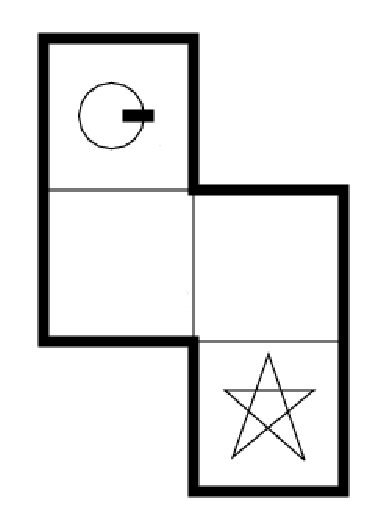
\includegraphics[scale=0.3]{problem-mini-hall}
\caption{\textit{Mini-hall} domain. Circle represents the agent, facing east. Starred cell is the goal state.}
\label{fig:problem-mini-hall}
\end{figure}


\begin{figure}[t]
\centering
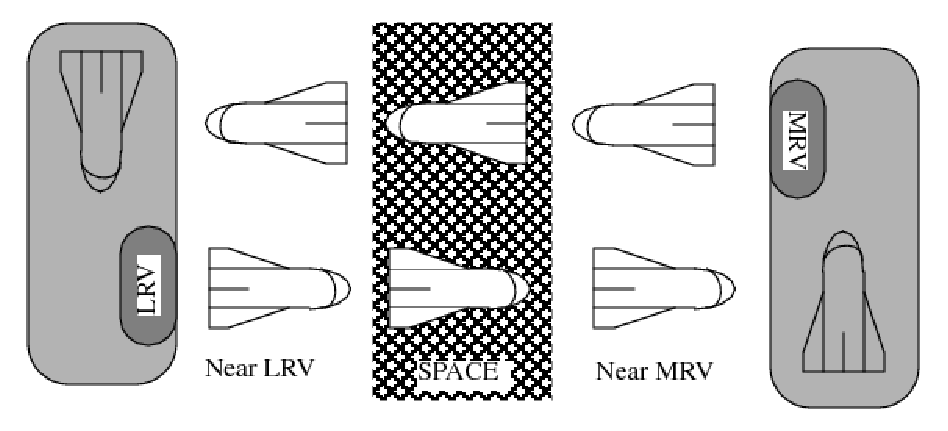
\includegraphics[scale=0.4]{problem-shuttle}
\caption{Illustration of \textit{Shuttle} problem. Each shuttle figure depicts a state. MRV stands for ``Most Recently Visited'' station, LRV stands for ``Least Recently Visited'' station.}
\label{fig:problem-shuttle}
\end{figure}


\subsection{Experiments and Discussion}
\label{sec:experiments}

Experiments are realized using four benchmark problems of different characteristics.

\textit{Mini-hall} \cite{littman_learning_1998} represents a simple problem setting with full determinism, representing the most trivial situation in our problem set (Figure \ref{fig:problem-mini-hall}).

\textit{Space shuttle docking problem (Shuttle)} \cite{chrisman_reinforcement_1992}  lacks a designated goal state, so the task is not inherently episodic. Although the problem size is small, unreliability of sensors and actions places the problem to a more difficult category than \textit{Mini-hall} in our set (Figure \ref{fig:problem-shuttle}).

\textit{Partially observable six room maze (PO-SixRoomMaze)}  is a limited observation variant of the original \textit{six room maze} problem \cite{girgin_improving_2010}.
In this version, agent is unable to perceive the exact state, but can perfectly sense the cell it occupies together with the content of the eight closest neighbouring cells. Importance of this problem is that it contains bottleneck states (doors), and is significantly larger than others (Figure \ref{fig:problem-room-maze}).

\textit{Rock sampling problem (RockSample[x,y])} \cite{smith_heuristic_2004} is a scalable problem that models rover science exploration, where $x$ is the dimension of square-shaped grid world and $y$ is number of rocks in the environment. There are two important properties of this domain, making it the most challenging problem of our set. (1) After sampling a rock, it becomes valueless, which means that the environment is non-stationary. (2) Observation space is very restricted, and observations are not reliable (Figure \ref{fig:problem-rock-sample3x3}).


\textit{Mini-hall} and \textit{Shuttle} problems are used as defined in their original references. Our set up for \textit{PO-SixRoomMaze} problem contains rooms of size $5\times5$, and for the $RockSample$ problem, $x$ and $y$ values are set to 3 and 3, respectively. 


\begin{figure}[t]
\centering
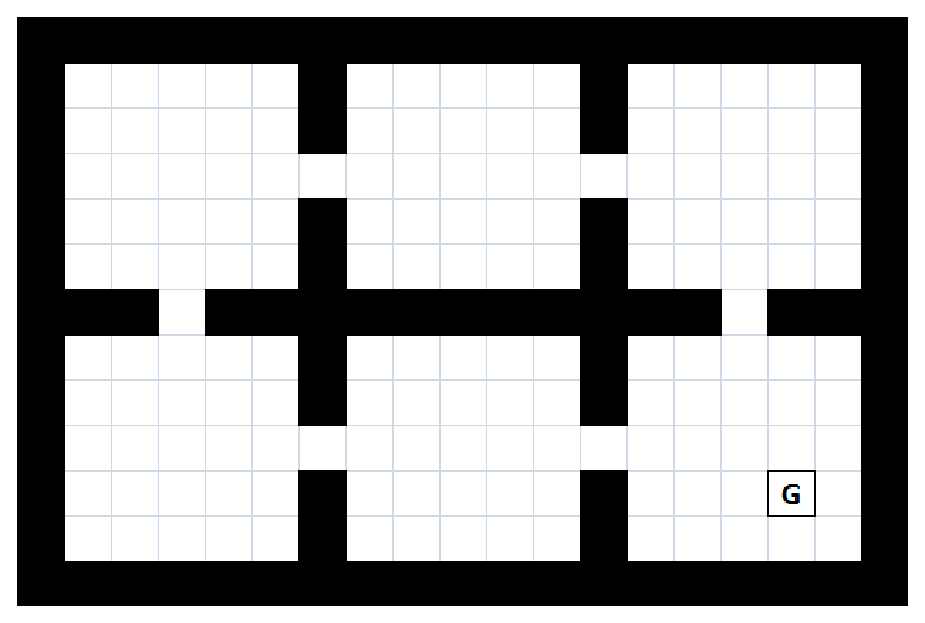
\includegraphics[scale=0.3]{problem-room-maze}
\caption{$2 \times 3$ room maze with rooms of size $5 \times 5$. Cell marked with G is the goal state.}
\label{fig:problem-room-maze}
\end{figure}

\begin{figure}[t]
\centering
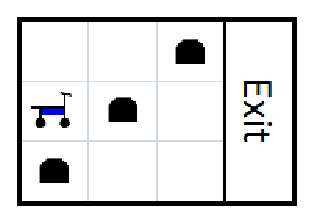
\includegraphics[scale=0.6]{problem-rock-sample3x3}
\caption{\textit{RockSample[3,3]} domain with a rover and three rocks.}
\label{fig:problem-rock-sample3x3}
\end{figure}

Sizes of problems in terms of state, action and observation set cardinalities are given in Table \ref{tab:problem_sizes}. 

\begin{table}[t]
\centering
	\caption{Problem sizes}
	\label{tab:problem_sizes}
	\begin{tabular}{ | l | l | l | l | }
		\hline
		\textbf{Problem} & $\mathbf{|S|}$ & $\mathbf{|A|}$ & $\mathbf{|\Omega|}$ \\ \hline
		\textit{Mini-hall} & 13 & 3 & 9 \\ \hline
		\textit{Shuttle} & 8 & 3 & 5 \\ \hline
		\textit{PO-SixRoomMaze} & 156 & 4 & 30 \\ \hline
		\textit{RockSample[3,3]} & 73 & 8 & 2 \\ \hline
	\end{tabular}
\end{table}



\subsubsection{Settings}

For all experiments, Modified-$\epsilon$-Greedy method in \cite{girgin_improving_2010} is updated by the required changes in action selection mechanism, as stated in Section \ref{sec:u-extended_seq_tree}.

Each problem is tested with Replicated-Q learning (without $D$-EST) and algorithm in Figure \ref{alg:replicatedQtree} (Replicated-Q learning with $D$-EST extension), and the results are compared. All the test runs are executed for varying number of episodes for each problem, depending on the convergence behaviour. Both algorithms are run 200 times for \textit{RockSample[3,3]} problem, and 50 times for others. The results are averaged over episodes of each run. 

Problems, except \textit{Shuttle}, are inherently episodic; i.e. the episode ends when a goal state is reached. For  \textit{Shuttle} problem, however, an episode is fixed by 250 steps, after which a new episode begins. In this problem, algorithm in Figure \ref{alg:replicatedQtree} is modified with ``reward-peak'' strategy, where maximum possible reward (instead of episode end) is used to trigger a sequence-tree update signal, possibly multiple times within an episode.

Default learning settings for problems are given in Table \ref{tab:default_rl_settings}. The only exception is, for the \textit{RockSample[3,3]}, $\epsilon$ value is set to 0.3, in order to promote exploration and achieve faster convergence, since Replicated-Q failed to converge in a reasonable time with the default settings. As a final note, for visual clarity, the plots of \textit{RockSample[3,3]} are smoothed.


\begin{table}[t]
\centering
	\caption{Default Settings}
	\label{tab:default_rl_settings}
	\begin{tabular}{ |l|l|}
		\hline
		\textbf{Parameter} & \textbf{Value} \\ \hline \hline
		$\alpha$ & 0.125 \\ \hline
		$\gamma$ & 0.9 \\ \hline
		$\epsilon$  & 0.1 \\ \hline
		$\psi_{decay}$ & 0.95 \\ \hline
		$\xi_{decay}$ & 0.99 \\ \hline
		$\psi_{treshold}$ & 0.01 \\ \hline
		$\xi_{treshold}$ & 0.01 \\ \hline
	\end{tabular}
\end{table}


\subsubsection{Results and Discussion}
\label{sec:experimental_results}

Results of the experiments are given in Figures \ref{fig:mini-hall}, \ref{fig:shuttle}, \ref{fig:room-maze} and \ref{fig:rock-sample}. Low ``number of steps per episode'' is the performance indicator for \textit{Mini-hall} and \textit{PO-SixRoomMaze} problems; while high ``cumulative reward per episode'' is the success criterion for \textit{Shuttle} and \textit{RockSample[3,3]} problems.


\begin{figure}[t]
\centering
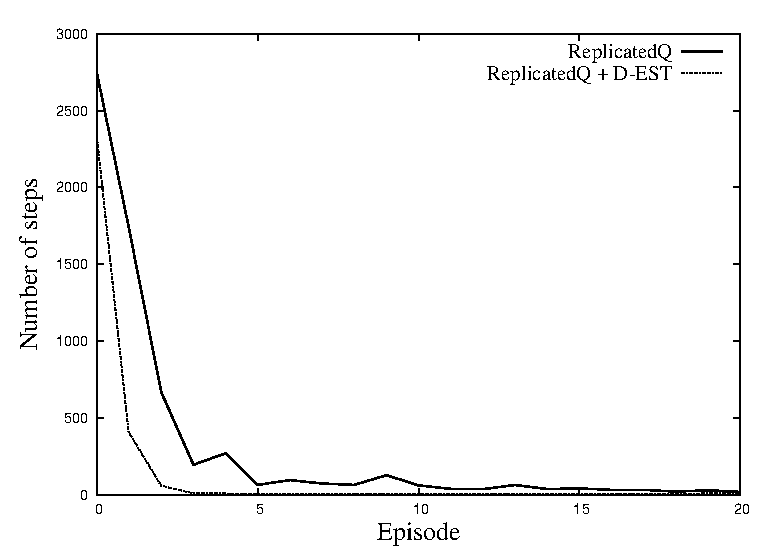
\includegraphics[width=\columnwidth]{results-mini-hall}
\caption{Experiment results for \textit{Mini-hall}.}
\label{fig:mini-hall}
\end{figure}


\begin{figure}[t]
\centering
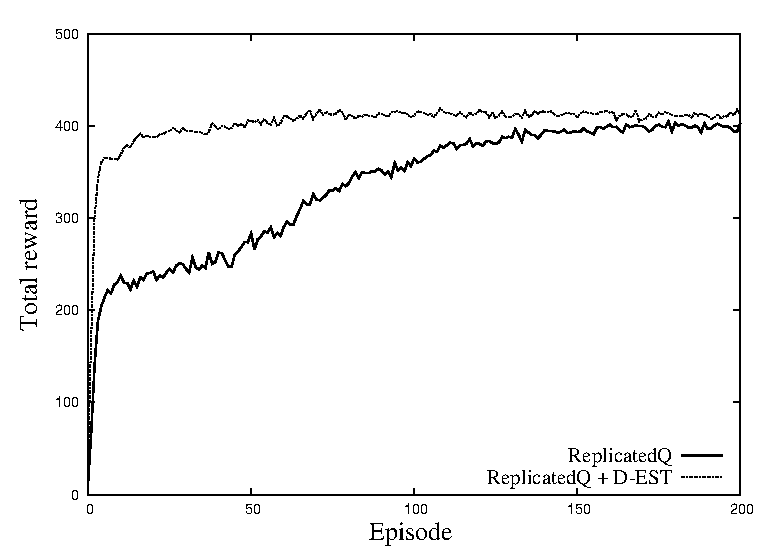
\includegraphics[width=\columnwidth]{results-shuttle}
\caption{Experiment results for \textit{Shuttle}.}
\label{fig:shuttle}
\end{figure}


\begin{figure}[t]
\centering
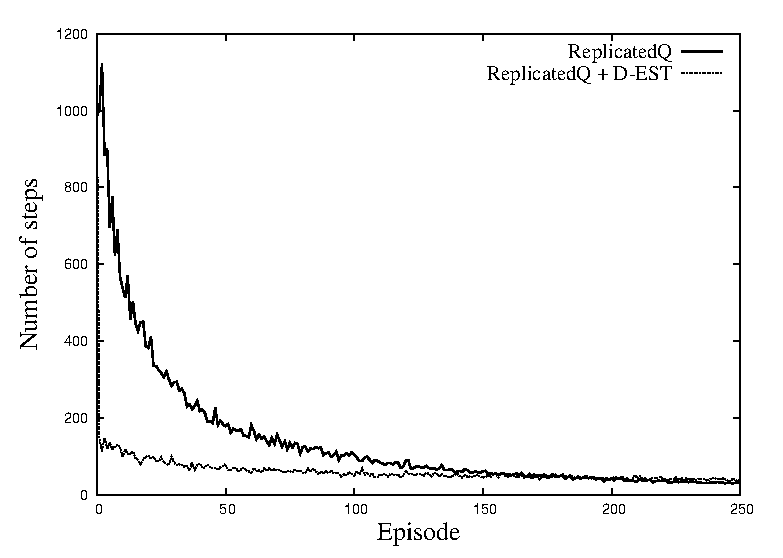
\includegraphics[width=\columnwidth]{results-room-maze}
\caption{Experiment results for \textit{PO-SixRoomMaze}.}
\label{fig:room-maze}
\end{figure}


\begin{figure}[t]
\centering
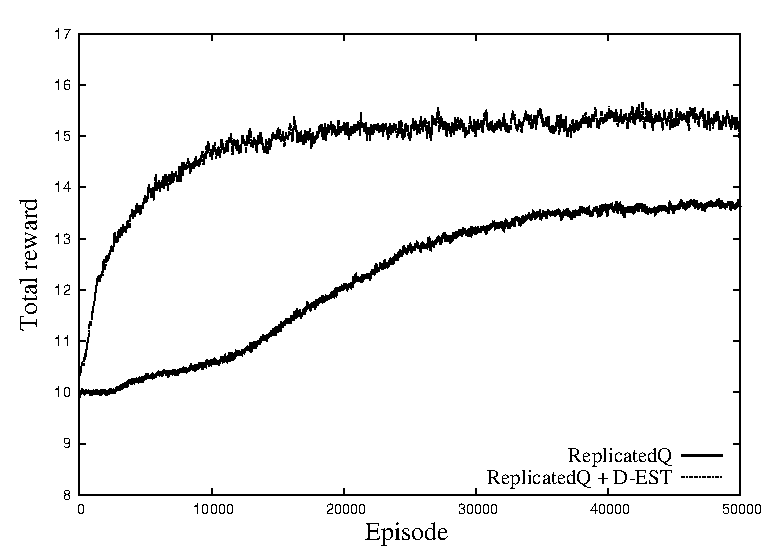
\includegraphics[width=\columnwidth]{results-rock-sample3x3}
\caption{Experiment results for \textit{RockSample[3,3]}.}
\label{fig:rock-sample}
\end{figure}

Results indicate that, given a partially observable problem, if it can be solved by a RL method, such as Replicated-Q Learning, a significant improvement can be achieved by $D$-EST abstraction. Although the term ``significance'' is not clear, observation and state transition function characteristics seem to play an important role. In that sense, even in relatively simpler problems \textit{Mini-hall} and \textit{PO-SixRoomMaze}, the proposed method outperforms the rapidly converging Replicated-Q case, meaning that the proposed discretization method produces approximations that effectively act as ``representative states'' within $D$-EST.

\textit{Shuttle} problem is highly non-deterministic. Nevertheless, ``reward-peak'' strategy effectively backs-up successful sub-policies, and immediately boosts learning performance, as seen in Figure \ref{fig:shuttle}. Similarly, a significant performance increase is achieved beginning from the early steps of learning for \textit{RockSample[3,3]} problem.


In general, the experiments show that $D$-EST abstraction successfully adapts the original EST mechanism to partial observability, and our discretization method performs reasonably well. There may be problems for which it would be necessary to ``design'' a specific discretization method, that is more suitable to domain characteristics than ours. When required, it is very easy to adapt $D$-EST abstraction and algorithm of Figure \ref{alg:replicatedQtree}, with the new discretization method designed upon a careful analysis of the domain.


\section{Conclusion}
\label{sec:conclusion}
This paper expands the existing ``Extended Sequence Tree'' abstraction method to cover POMDPs through discretization of belief space, and proposes a belief discretization method for it that is simple and effective. Effectiveness of resulting method and discretization scheme are shown via experimentation over four partially observable problem domains, and the results are discussed.

Possible future research directions include experimentation of other discretization schema, extending EST to include other partially observable RL paradigms (like gradient descent based algorithms), and inclusion of some  characteristic information (rewards, state-action values, etc.) as clues for higher accuracy.


% conference papers do not normally have an appendix


% use section* for acknowledgement
%\section*{Acknowledgment}
%The authors would like to thank...
%more thanks here


% trigger a \newpage just before the given reference
% number - used to balance the columns on the last page
% adjust value as needed - may need to be readjusted if
% the document is modified later
%\IEEEtriggeratref{17}
% The "triggered" command can be changed if desired:
%\IEEEtriggercmd{\enlargethispage{-5in}}

% references section

% can use a bibliography generated by BibTeX as a .bbl file
% BibTeX documentation can be easily obtained at:
% http://www.ctan.org/tex-archive/biblio/bibtex/contrib/doc/
% The IEEEtran BibTeX style support page is at:
% http://www.michaelshell.org/tex/ieeetran/bibtex/
\bibliographystyle{IEEEtran}
% argument is your BibTeX string definitions and bibliography database(s)
\bibliography{IEEEabrv,referencesNoURL}
%
% <OR> manually copy in the resultant .bbl file
% set second argument of \begin to the number of references
% (used to reserve space for the reference number labels box)
%\begin{thebibliography}{1}

%\bibitem{IEEEhowto:kopka}
%H.~Kopka and P.~W. Daly, \emph{A Guide to \LaTeX}, 3rd~ed.\hskip 1em plus
%  0.5em minus 0.4em\relax Harlow, England: Addison-Wesley, 1999.

%\end{thebibliography}

% that's all folks
\end{document}


